\documentclass{article}
\usepackage{fullpage}
\usepackage{amsmath,amssymb,amsfonts}
\usepackage{graphicx}
\usepackage{natbib}
\usepackage[colorinlistoftodos]{todonotes}

\def\R{{\mathbb{R}}}
\def\pr{{\rm Pr}}
\def\E{{\mathbb E}}
\def\X{{\mathcal X}}
\def\Y{{\mathcal Y}}
\def\H{{\mathcal H}}
\def\G{{\mathcal G}}
\def\B{{\mathcal B}}
\def\bias{{\rm bias}}
\def\supp{{\rm supp}}

\newtheorem{thm}{Theorem}
\newtheorem{lemma}[thm]{Lemma}
\newtheorem{cor}[thm]{Corollary}
\newtheorem{claim}[thm]{Claim}
\newtheorem{defn}[thm]{Definition}
\newtheorem{assump}{Assumption}
\newtheorem{open}{Open problem}
\newenvironment{proof}{\noindent {\sc Proof:}}{$\Box$ \medskip}

\DeclareMathOperator*{\argmax}{arg\,max}

\newcommand{\new}[1]{{\color{red} #1}}
\newcommand{\shay}[1]{{\color{purple} {\bf Shay:} #1}}


\title{An adaptive nearest neighbor rule for classification}

\begin{document}

\maketitle

\section{Introduction}

We introduce an adaptive nearest neighbor classification rule. Given a training set with labels $\{0,1\}$ and a query point $x$, it makes a prediction based on the training points closest to $x$, rather like the $k$-nearest neighbor rule. However, the value of $k$ that it uses can vary from query to query. Specifically, if there are $n$ training points, then for any query $x$, the smallest $k$ is sought for which the $k$ points closest to $x$ have labels whose average is either greater than $1/2 + \Delta(n,k)$, in which case the prediction is $1$, or less than $1/2 - \Delta(n,k)$, in which case the prediction is 0; and if no such $k$ exists, then a label is chosen at random. Here $\Delta(n,k) \sim \sqrt{(\log n)/k}$ corresponds to a confidence interval for the average label in the region around the query.

We study this rule in the standard framework in which all data are i.i.d.\ draws from some unknown underlying distribution $P$ on $\X \times \Y$, where $\X$ is the data space and $\Y$ is the label space. We take $\X$ to be a separable metric space, with distance function $d: \X \times \X \rightarrow \R$, and we take $\Y = \{0,1\}$. We can decompose $P$ into the marginal distribution $\mu$ on $\X$ and the conditional distribution of the label at each point $x$: if $(X,Y)$ represents a random draw from $P$, define $\eta(x) = \pr(Y = 1 | X = x)$. In this terminology, the Bayes-optimal classifier is the rule $g^*: \X \rightarrow \{0,1\}$ given by
$$ g^*(x) = 
\left\{
\begin{array}{ll}
1 & \mbox{$\eta(x) > 1/2$} \\
0 & \mbox{otherwise}
\end{array}
\right.
$$
and its error rate is $R^* = \E_{X \sim \mu} \min(\eta(X), 1- \eta(X))$. A variety of nonparametric classification schemes are known to have error rates that converge asymptotically to $R^*$. These include $k$-nearest neighbor (henceforth, $k$-NN) rules in which $k$ grows with the number of training points $n$ according to a suitable schedule $(k_n)$, under certain technical conditions on the metric measure space $(\X, d, \mu)$.

In this paper, we are interested in consistency as well as rates of convergence. In particular, we find that the adaptive nearest neighbor rule is also asymptotically consistent (under the same technical conditions) while converging at a rate that is at least as good as, and in some cases better than, that of $k$-NN under any schedule $(k_n)$.

Intuitively, one of the advantages of $k$-NN over nonparametric classifiers that use a fixed bandwidth or radius, such as Parzen window or kernel density estimators, is that $k$-NN automatically adapts to fluctuations in the marginal distribution $\mu$: in regions with large $\mu$, the $k$ nearest neighbors lie close to the query point, while in regions with small $\mu$, the $k$ nearest neighbors can be further afield. The adaptive NN rule that we propose goes further: it also adapts to fluctuations in $\eta$. In certain regions of the input space, where $\eta$ is close to $1/2$, an accurate prediction would need large $k$. In other regions, where $\eta$ is near 0 or 1, a small $k$ would suffice, and in fact, a larger $k$ might be detrimental because neighboring regions might be labeled differently. See Figure~\ref{fig:rationale} for one such example. A $k$-NN classifier is forced to pick a single value of $k$ that trades off between these two contingencies. Our adaptive NN rule, however, can pick the right $k$ in each neighborhood separately.

\begin{figure}
\begin{center}
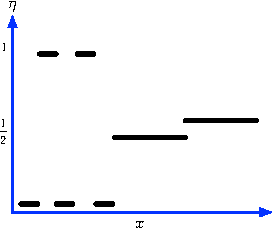
\includegraphics[width=3in]{adaptive-rationale.pdf}
\end{center}
\caption{For values of $x$ on the left half of the shown interval, the conditional probability function $\eta(x)$ is close to 0 or 1, and thus a small value of $k$ will yield an accurate prediction. Larger $k$ will not do as well, because they may run into neighboring regions with different labels. For values of $x$ on the right half of the interval, $\eta(x)$ is close to $1/2$, and thus large $k$ is essential for accurate prediction.}
\label{fig:rationale}
\end{figure}


\section{An adaptive nearest neighbor rule}

Let $(\X,d)$ be a separable metric space and let $\Y = \{0,1\}$. Suppose we are given a labeled data set $(x^{(1)}, y^{(1)}), \ldots, (x^{(n)}, y^{(n)}) \in \X \times \Y$.

For any set $S \subset \X$, define the empirical mass of $S$ to be
\begin{equation}
\mu_n(S) = \frac{|\{x^{(i)} \in S\}|}{n} ,
\label{eq:empirical-mass}
\end{equation}
and define the empirical label bias of $S$ as
\begin{equation}
\bias_n(S) = \frac{|\{x^{(i)} \in S: y^{(i)} = 1\}|}{n \, \mu_n(S)} - \frac{1}{2}.
\label{eq:empirical-bias}
\end{equation}
\shay{This equation is unintuitive. I suggest to introduce a notation for conditional empirical probability $\mu_n(\cdot \bar S)$ and use it.}

Let $0 < \delta < 1$ be any pre-specified confidence parameter. Given a query point $x$, we make a prediction $\{0,1,?\}$, where $?$ denotes ``don't know'', according to the following rule:
\begin{itemize}
\item Find the smallest ball $B$ centered at $x$ whose empirical bias has absolute value at least
$$ \Delta(n,k) = c_1 \sqrt{\frac{d_o \log n + \log (1/\delta)}{k}}, $$
where $k$ is the number of points $x^{(i)}$ in $B$. The constants $c_1$ and $d_o$ are from Lemma~\ref{lemma:bias} below.
\item If no such ball exists: predict ?. Otherwise, predict the majority label in $B$.
\end{itemize}
Let $g_n: \X \rightarrow \{0,1,?\}$ denote this classifier.

\section{Large deviation bounds}

Suppose that all data $(x,y)$ is obtained by independent draws from an underlying distribution $P$ on $\X \times \Y$. For $(X,Y) \sim P$, define $\mu$ to be the marginal distribution of $X$, that is,
$$ \mu(S) = \pr(X \in S) $$
for measurable sets $S$. Let $\eta$ be the conditional probability distribution of $Y$ given $x$,
$$ \eta(x) = \pr(Y = 1| X = x) .$$
For measurable $S$, let $\eta(S)$ denote the average $\eta$-value, that is,
$$ \eta(S) = \pr(Y = 1| X \in S) = \frac{1}{\mu(S)} \int_S \eta \ d \mu .$$

Suppose we draw $n$ points $(x^{(1)}, y^{(1)}), \ldots, (x^{(n)}, y^{(n)})$ from $P$. If $n$ is reasonably large, we would expect the empirical mass $\mu_n(S)$ of any set $S \subset \X$, as defined in (\ref{eq:empirical-mass}), to be close to its probability mass under $\mu$. The following lemma, from Chaudhuri-Dasgupta (2010), quantifies one particular aspect of this.
\begin{lemma}
There is a universal constant $c_o$ such that the following holds. Let $\B$ be any class of measurable subsets of $\X$ of VC dimension $d_o$. Pick any $0 < \delta < 1$. Then with probability at least $1-\delta^2/2$ over the choice of $(x^{(1)}, y^{(1)}), \ldots, (x^{(n)}, y^{(n)})$, for all $B \in \B$ and for any integer $k$, we have
$$ \mu(B) \geq \frac{k}{n} + \frac{c_o}{n} \max \left( k, d_o \log \frac{n}{\delta} \right)
\ \ \implies \ \ 
\mu_n(B) \geq \frac{k}{n} .$$
\label{lemma:points-in-balls}
\end{lemma}

Likewise, we would expect the empirical bias of a set $S \subset \X$, as defined in (\ref{eq:empirical-bias}), to be close to its true bias,
$$ \bias(S) = \frac{\pr(Y = 1, X \in S)}{\pr(X \in S)} - \frac{1}{2} .$$
This is defined when $\mu(S) > 0$ and lies in the range $[-1/2,1/2]$.

\begin{lemma}[Shay's bound]
There is a universal constant $c_1$ for which the following holds. Let $\B$ be a class of subsets of $\X$ with VC dimension $d_o$. Pick any $0 < \delta < 1$. Then with probability at least $1-\delta^2/2$ over the choice of $(x^{(1)}, y^{(1)}), \ldots, (x^{(n)}, y^{(n)})$, for all $B \in \B$,
  $$ \left| \bias_n(B) - \bias(B) \right| \ \leq \ \Delta(n, k(B)) $$
where $k(B) = |\{i: x^{(i)} \in B\}|$ is the number of points inside $B$ and 
\begin{equation}
\Delta(n,k) = c_1 \sqrt{\frac{d_o \log n + \log (1/\delta)}{k}} .
\label{eq:delta-defn}
\end{equation}
\label{lemma:bias}
\end{lemma}

\section{Fine-grained analysis and universal consistency}
\label{sec:universal-consistency}

Define the support of the marginal distribution $\mu$ to be
$$ \supp(\mu) = \{x \in \X: \mbox{$\mu(B(x,r)) > 0$ for all $r > 0$}\} .$$

For any $x \in \supp(\mu)$ and $p > 0$, let $r_p(x)$ denote the smallest radius such that the probability mass of $B(x, r_p(x))$ is at least $p$:
$$ r_p(x) = \inf \{r > 0: \mu(B(x,r)) \geq p \} .$$
Then $\mu(B(x,r_p(x))) \geq p$.

We now characterize the region of $\X$ that the adaptive rule is likely to correctly classify as having label $1$, given $n$ training points. It is the set $\X^+_n$ of points $x \in \supp(\mu)$, with $\eta(x) > 1/2$, for which there exists $p_x > 0$ such that:
\begin{itemize}
\item $\eta(B(x,r_{p_x}(x))) \geq \frac{1}{2} + c_2 \sqrt{\frac{\log (n/\delta)}{np_x}}$, where $c_2 = \max(2c_1, 1/2) \sqrt{1+c_o}$. 
\shay{Should it be $\eta$ here?} 
\item $\eta(B(x,r)) \geq 1/2$ for all $0 < r \leq r_{p_x}(x)$. 
\end{itemize}
The set $\X^-_n$ can be defined symmetrically, as consisting of $x \in \supp(\mu)$ with $\eta(x) < 1/2$, and for which there exists $p_x > 0$ such that:
\begin{itemize}
\item $\eta(B(x,r_{p_x}(x))) \leq \frac{1}{2} - c_2 \sqrt{\frac{\log (n/\delta)}{np_x}}$. 
\item $\eta(B(x,r)) \leq 1/2$ for all $0 < r \leq r_{p_x}(x)$. 
\end{itemize}

\begin{lemma}
Fix any $x \in \X^+_n \cup \X^-_n$. Pick $n$ training points at random from $P$. With probability at least $1-\delta^2$ over the choice of training data, the adaptive $k$-NN rule will predict 1 if $x \in \X^+_n$, or $0$ if $x \in \X^-_n$.
\label{lemma:good-sets}
\end{lemma}
\begin{proof}
Fix any $x \in \X^+_n$; the case of $x \in \X^-_n$ is symmetric. The set $\B$ of all balls centered at $x$ is easily seen to have VC dimension 1. By Lemmas~\ref{lemma:points-in-balls} and \ref{lemma:bias}, we have that with probability at least $1-\delta^2$, the following two properties hold for all $B \in \B$:
\begin{enumerate}
\item For any integer $k$, we have $\mu_n(B) \geq k/n$ whenever $n \mu(B) \geq k + c_o \max(k, \log (n/\delta))$.
\item $|\bias_n(B) - \bias(B)| \leq \Delta(n, n \mu_n(B))$.
\end{enumerate}
Assume henceforth that these hold.

Let $p = p_x$ be as specified in the definition of $\X^+_n$. Set $k = np/(1 + c_o)$. We first observe that $k \geq \log (n/\delta)$. This is because the definition of $p$ implies $c_2 \sqrt{\log (n/\delta)/(np)} \leq 1/2$ and thus $np \geq 4 c_2^2 \log (n/\delta) \geq (1+c_o) \log (n/\delta)$.

As a result, $np \geq k + c_o \max(k, \log (n/\delta))$. Thus, by property 1, the ball $B = B(x, r_p(x))$ has $\mu_n(B) \geq k/n$. This means, in turn, that by property 2,
\begin{align*}
\bias_n(B) &\geq \bias(B) - \Delta(n, k) \\
&\geq c_2 \sqrt{\frac{\log (n/\delta)}{np}} - c_1 \sqrt{\frac{\log (n/\delta)}{k}} \\
&\geq 2c_1 \sqrt{\frac{\log (n/\delta)}{k}} - c_1 \sqrt{\frac{\log (n/\delta)}{k}} \\
&= c_1 \sqrt{\frac{\log (n/\delta)}{k}} \geq \Delta(n, n \mu_n(B)) .
\end{align*}
Thus ball $B$ would trigger a prediction of $1$.

At the same time, for any ball $B' = B(x, r)$ with $r < r_p(x)$,
$$ \bias_n(B') \geq \bias(B') - \Delta(n, n \mu_n(B')) > -\Delta(n, n \mu_n(B')) $$
and thus no such ball will trigger a prediction of $0$. Therefore, the prediction at $x$ must be $1$.
\end{proof}

Based on this result, it makes sense to define the {\it effective boundary} when there are $n$ data points as 
$$ \partial_n = \X \setminus (\X^+_n \cup \X^-_n) .$$
Then we have the following bound on the error rate of the adaptive nearest neighbor classifier.
\begin{thm}
Pick any $0 < \delta < 1$. With probability at least $1-\delta$ over the choice of training points,
$$ \pr_{X}(g_n(X) \neq g^*(X)) \ \leq \ \delta + \mu(\partial_n) .$$
Here $g_n$ is the adaptive nearest neighbor classifier based on the $n$ training points and $g^*$ is the Bayes-optimal classifier. 
\label{thm:general-error-bound}
\end{thm}
\begin{proof}
From Lemma~\ref{lemma:good-sets}, we have that for any $x \in \X^+_n \cup \X^-_n$, 
$$ \pr_n(g_n(x) \neq g^*(x)) \leq \delta^2 ,$$
where $\pr_n$ denotes probability over the choice of training points. Thus, for $X \sim \mu$,
$$ \E_n \E_X 1(g_n(X) \neq g^*(X) | X \in \X^+_n \cup \X^-_n) \leq \delta^2 ,$$
and by Markov's inequality,
$$ \pr_n [\pr_X (g_n(X) \neq g^*(X) |  X \in \X^+_n \cup \X^-_n) \geq \delta] \leq \delta.$$
Thus, with probability at least $1-\delta$ over the training set,
$$\pr_X (g_n(X) \neq g^*(X) |  X \in \X^+_n \cup \X^-_n) \leq \delta$$
and
$$ \pr_X(g_n(X) \neq g^*(X)) 
\ \leq \ \delta \ \pr(X \in \X^+_n \cup X^-_n) + \pr(X \not\in \X^+_n \cup X^-_n)
\ \leq \ \delta + \mu(\partial_n) .$$
\end{proof}

It follows, using the same argument as in Chaudhuri-Dasgupta (2014), that the adaptive nearest neighbor rule is universally consistent as long as the metric space $(\X, d, \mu)$ satisfies Lebesgue's differentiation condition: that is, for any bounded measurable $f: \X \rightarrow \R$,
$$ \lim_{r \downarrow 0} \frac{1}{\mu(B(x,r))} \int_{B(x,r)} f \ d\mu = f(x) .$$
This holds in any finite-dimensional normed space, or any doubling metric space.

\section{Rates of convergence}

We now provide finite-sample rates of convergence of the adaptive nearest neighbor rule. For simplicity, we give convergence rates that are specific to any query point $x$ and that depend on a suitable notion of the ``margin'' of distribution $P$ around $x$.

Pick any $p, \gamma > 0$. We define a point $x \in \X$ as $(p, \gamma)$-salient if 
\begin{itemize}
\item either $\eta(x') \geq 1/2 + \gamma$ for all $x' \in B(x, r_p(x))$
\item or $\eta(x') \leq 1/2 - \gamma$ for all $x' \in B(x, r_p(x))$.
\end{itemize}
If $\eta$ and $\mu$ are continuous then for any $x \in \X$ with $\eta(x) \neq 1/2$, there must be some sufficiently small $p, \gamma > 0$ for which this is true.

Let $S_{p, \gamma}$ be the set of all $(p, \gamma)$-salient points. We then define the {\it margin} of any $x \in \X$ as
$$ m(x) = \max_{S_{p, \gamma} \ni x} p \gamma^2 .$$
Notice that if 
$$ n \geq \frac{1}{m(x)} \ln \frac{1}{m(x)} ,$$
then $x \in \X_n^+ \cup \X_n^-$, as defined in Section~\ref{sec:universal-consistency}, and thus $x$ is very likely to be correctly classified by the adaptive nearest neighbor rule, given a training set of $n$ points.


\noindent{\bf Earlier notes:}

In order that a point $x$ be classified correctly for a small value of $n$ it suffices that there is a ball $B$ centered at $x$ with significant bias and significant probability. More precisely, if there is a ball of probability $p$ around $x$ for which there is a uniform bias of $\gamma$ then probability that the adaptive NN rule is incorrect 
on $x$ is $\exp(-c k \gamma^2) \approx \exp(-c p n \gamma^2)$

We formalize this as follows.

Let $\X_{\alpha}^+$ be the set of points $x \in \X$ such that there exist $p,\gamma>0$ such that $p \gamma^2 \geq \alpha$ and  $\forall x' \in B(x,p)$ $\eta(x')\geq \gamma$. $\X_{\alpha}^-$ is defined similarly.

Then we have the following theorem:
\begin{thm}
For all $\alpha>0$ and all $x \in \X_{\alpha}^+ \cup \X_{\alpha}^-$ the probability that AKNN predicts incorrectly on $x$ is upper bounded by $\exp(-c n \alpha)$.
\end{thm}

\end{document}
